% Options for packages loaded elsewhere
\PassOptionsToPackage{unicode}{hyperref}
\PassOptionsToPackage{hyphens}{url}
%
\documentclass[
  12pt,
  a4paper,
]{scrreprt}
\usepackage{amsmath,amssymb}
\usepackage{setspace}
\usepackage{iftex}
\ifPDFTeX
  \usepackage[T1]{fontenc}
  \usepackage[utf8]{inputenc}
  \usepackage{textcomp} % provide euro and other symbols
\else % if luatex or xetex
  \usepackage{unicode-math} % this also loads fontspec
  \defaultfontfeatures{Scale=MatchLowercase}
  \defaultfontfeatures[\rmfamily]{Ligatures=TeX,Scale=1}
\fi
\usepackage{lmodern}
\ifPDFTeX\else
  % xetex/luatex font selection
  \setmainfont[Ligatures=TeX]{PT Serif}
  \setsansfont[Ligatures=TeX,Scale=MatchLowercase]{PT Sans}
  \setmonofont[Scale=MatchLowercase,Scale=0.9]{PT Mono}
\fi
% Use upquote if available, for straight quotes in verbatim environments
\IfFileExists{upquote.sty}{\usepackage{upquote}}{}
\IfFileExists{microtype.sty}{% use microtype if available
  \usepackage[]{microtype}
  \UseMicrotypeSet[protrusion]{basicmath} % disable protrusion for tt fonts
}{}
\usepackage{xcolor}
\usepackage{longtable,booktabs,array}
\usepackage{calc} % for calculating minipage widths
% Correct order of tables after \paragraph or \subparagraph
\usepackage{etoolbox}
\makeatletter
\patchcmd\longtable{\par}{\if@noskipsec\mbox{}\fi\par}{}{}
\makeatother
% Allow footnotes in longtable head/foot
\IfFileExists{footnotehyper.sty}{\usepackage{footnotehyper}}{\usepackage{footnote}}
\makesavenoteenv{longtable}
\usepackage{graphicx}
\makeatletter
\def\maxwidth{\ifdim\Gin@nat@width>\linewidth\linewidth\else\Gin@nat@width\fi}
\def\maxheight{\ifdim\Gin@nat@height>\textheight\textheight\else\Gin@nat@height\fi}
\makeatother
% Scale images if necessary, so that they will not overflow the page
% margins by default, and it is still possible to overwrite the defaults
% using explicit options in \includegraphics[width, height, ...]{}
\setkeys{Gin}{width=\maxwidth,height=\maxheight,keepaspectratio}
% Set default figure placement to htbp
\makeatletter
\def\fps@figure{htbp}
\makeatother
\setlength{\emergencystretch}{3em} % prevent overfull lines
\providecommand{\tightlist}{%
  \setlength{\itemsep}{0pt}\setlength{\parskip}{0pt}}
\setcounter{secnumdepth}{5}
\ifLuaTeX
\usepackage[bidi=basic]{babel}
\else
\usepackage[bidi=default]{babel}
\fi
\babelprovide[main,import]{russian}
\ifPDFTeX
\else
\babelfont[russian]{rm}{PT Serif}
\fi
\babelprovide[import]{english}
% get rid of language-specific shorthands (see #6817):
\let\LanguageShortHands\languageshorthands
\def\languageshorthands#1{}
\usepackage{indentfirst}
\usepackage{float}
\floatplacement{figure}{H}

%% pandoc-tablenos: required package
\usepackage{caption}

%% pandoc-tablenos: environment to disable table caption prefixes
\makeatletter
\newcounter{tableno}
\newenvironment{tablenos:no-prefix-table-caption}{
  \caption@ifcompatibility{}{
    \let\oldthetable\thetable
    \let\oldtheHtable\theHtable
    \renewcommand{\thetable}{tableno:\thetableno}
    \renewcommand{\theHtable}{tableno:\thetableno}
    \stepcounter{tableno}
    \captionsetup{labelformat=empty}
  }
}{
  \caption@ifcompatibility{}{
    \captionsetup{labelformat=default}
    \let\thetable\oldthetable
    \let\theHtable\oldtheHtable
    \addtocounter{table}{-1}
  }
}
\makeatother
\ifLuaTeX
  \usepackage{selnolig}  % disable illegal ligatures
\fi
\usepackage[style=gost-numeric,parentracker=true,backend=biber,hyperref=auto,language=auto,autolang=other*,citestyle=gost-numeric]{biblatex}
\addbibresource{bib/cite.bib}
\IfFileExists{bookmark.sty}{\usepackage{bookmark}}{\usepackage{hyperref}}
\IfFileExists{xurl.sty}{\usepackage{xurl}}{} % add URL line breaks if available
\urlstyle{same}
\hypersetup{
  pdftitle={Отчёт по лабораторной работе №1 Математическое моделирование},
  pdfauthor={Выполнила: Малашенко Марина Владимировна, НФИбд-01-20, 1032202459},
  pdflang={ru-RU},
  hidelinks,
  pdfcreator={LaTeX via pandoc}}

\title{Отчёт по лабораторной работе №1\\
Математическое моделирование}
\usepackage{etoolbox}
\makeatletter
\providecommand{\subtitle}[1]{% add subtitle to \maketitle
  \apptocmd{\@title}{\par {\large #1 \par}}{}{}
}
\makeatother
\subtitle{Настройка рабочего пространства. Система контроля версий Git.
Язык разметки Markdown}
\author{Выполнила: Малашенко Марина Владимировна,\\
НФИбд-01-20, 1032202459}
\date{}

\begin{document}
\maketitle

\renewcommand*\contentsname{Содержание}
{
\setcounter{tocdepth}{2}
\tableofcontents
}
\listoffigures
\setstretch{1.5}
\hypertarget{ux446ux435ux43bux44c-ux440ux430ux431ux43eux442ux44b}{%
\chapter{Цель
работы}\label{ux446ux435ux43bux44c-ux440ux430ux431ux43eux442ux44b}}

Настроить рабочее пространство для лабораторной работы. Изучить систему
контроля версий Git и язык разметки Markdown.

\hypertarget{ux437ux430ux434ux430ux43dux438ux435}{%
\chapter{Задание}\label{ux437ux430ux434ux430ux43dux438ux435}}

Создать директорию, создать репозиторий, настроить связь между своим
компьютером и GitHub по SSH-ключу. При помощи Makefile сконвертировать
из файла .md файлы отчетов в форматах docx и pdf. Запушить все готовые
отчеты на Github.

\hypertarget{ux442ux435ux43eux440ux435ux442ux438ux447ux435ux441ux43aux43eux435-ux432ux432ux435ux434ux435ux43dux438ux435}{%
\chapter{Теоретическое
введение}\label{ux442ux435ux43eux440ux435ux442ux438ux447ux435ux441ux43aux43eux435-ux432ux432ux435ux434ux435ux43dux438ux435}}

Git — система управления версиями с распределенной архитектурой. В
отличие от некогда популярных систем вроде CVS и Subversion (SVN), где
полная история версий проекта доступна лишь в одном месте, в Git каждая
рабочая копия кода сама по себе является репозиторием. Это позволяет
всем разработчикам хранить историю изменений в полном объеме.

Markdown — облегчённый язык разметки, созданный с целью обозначения
форматирования в простом тексте, с максимальным сохранением его
читаемости человеком, и пригодный для машинного преобразования в языки
для продвинутых публикаций (HTML, Rich Text и других).

\begin{tablenos:no-prefix-table-caption}

\begin{longtable}[]{@{}
  >{\raggedright\arraybackslash}p{(\columnwidth - 2\tabcolsep) * \real{0.1014}}
  >{\raggedright\arraybackslash}p{(\columnwidth - 2\tabcolsep) * \real{0.8986}}@{}}
\toprule\noalign{}
\begin{minipage}[b]{\linewidth}\raggedright
Название команды
\end{minipage} & \begin{minipage}[b]{\linewidth}\raggedright
Описание команды
\end{minipage} \\
\midrule\noalign{}
\endhead
\bottomrule\noalign{}
\endlastfoot
\texttt{git\ clone} & Клонирование репозитория на ПК \\
\texttt{git\ commit\ -m\ "Initial\ Commit"} & Оставление коммита \\
\texttt{git\ push} & Загрузка изменений на гит \\
\texttt{make} & Конвертация файла .md \\
\end{longtable}

\end{tablenos:no-prefix-table-caption}

\hypertarget{ux432ux44bux43fux43eux43bux43dux435ux43dux438ux435-ux43bux430ux431ux43eux440ux430ux442ux43eux440ux43dux43eux439-ux440ux430ux431ux43eux442ux44b}{%
\chapter{Выполнение лабораторной
работы}\label{ux432ux44bux43fux43eux43bux43dux435ux43dux438ux435-ux43bux430ux431ux43eux440ux430ux442ux43eux440ux43dux43eux439-ux440ux430ux431ux43eux442ux44b}}

\textbf{1.} Создадим директорию на своем компьютере по шаблону:

\begin{figure}
\centering
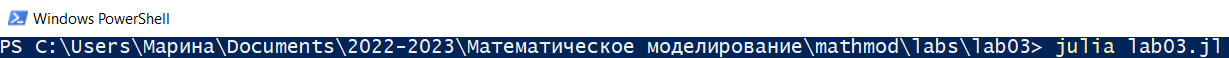
\includegraphics{./tex2pdf.-cbf55669a78d292a/image/1.PNG}
\caption{(рис. 1. Шаблон директории)}
\end{figure}

\textbf{2.} Авторизируемся на Github:

\begin{figure}
\centering
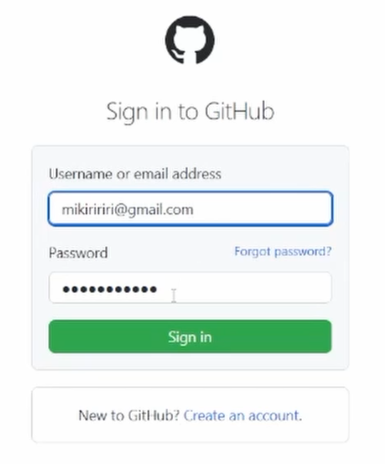
\includegraphics{./tex2pdf.-cbf55669a78d292a/image/2.PNG}
\caption{(рис. 2. Авторизация)}
\end{figure}

\textbf{3.} Перейдем к шаблону репозитория и создадим по нему свой новый
репозиторий:

\begin{figure}
\centering
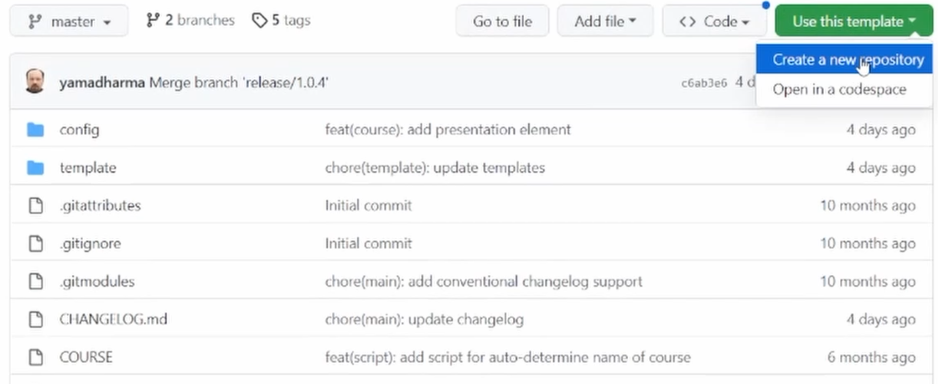
\includegraphics{./tex2pdf.-cbf55669a78d292a/image/3.PNG}
\caption{(рис. 3. Шаблон репозитория)}
\end{figure}

\textbf{4.} Создадим и настроим репозиторий:

\begin{figure}
\centering
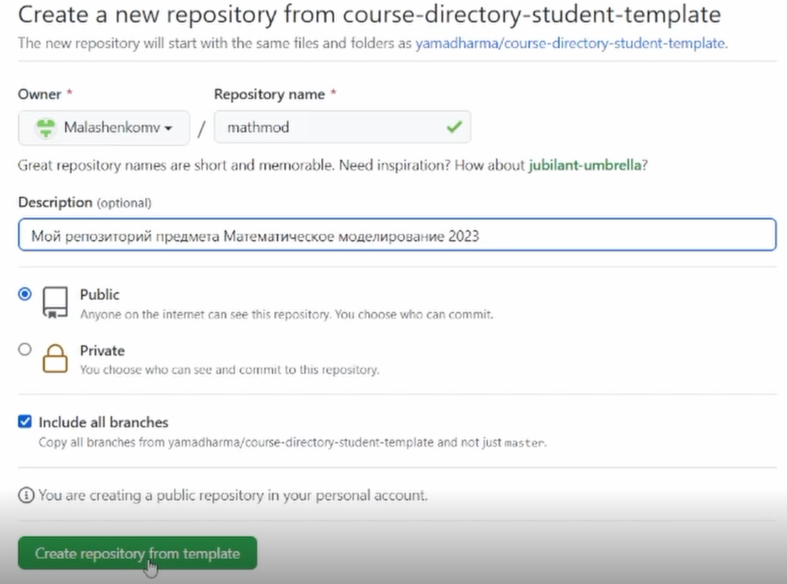
\includegraphics{./tex2pdf.-cbf55669a78d292a/image/4.PNG}
\caption{(рис. 4. Создание репозитория)}
\end{figure}

\textbf{5.} Установим make:

\begin{figure}
\centering
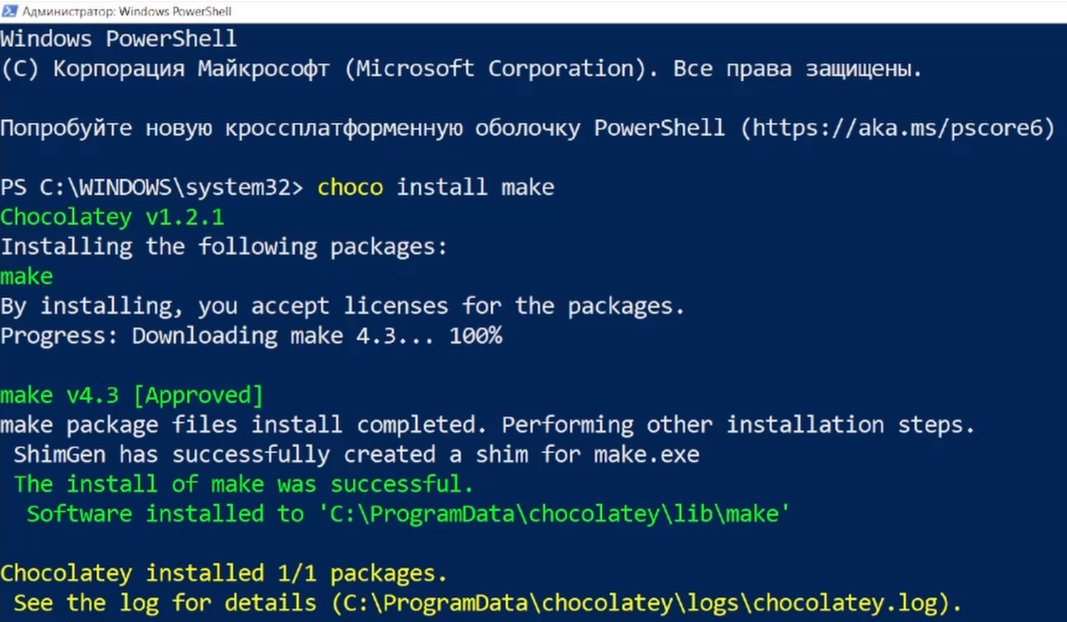
\includegraphics{./tex2pdf.-cbf55669a78d292a/image/5.PNG}
\caption{(рис. 5. Установка make)}
\end{figure}

\textbf{6.} Установим git:

\begin{figure}
\centering
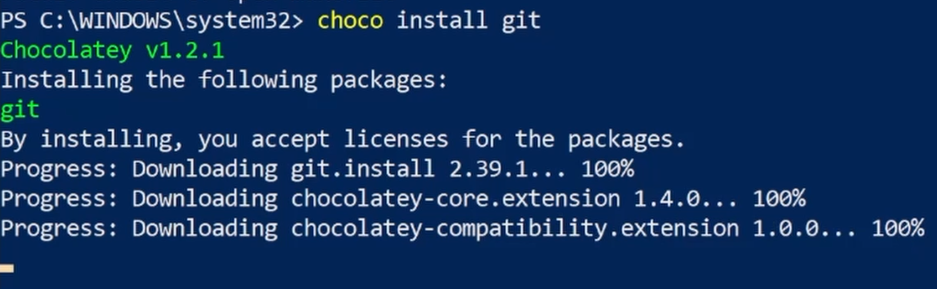
\includegraphics{./tex2pdf.-cbf55669a78d292a/image/6.PNG}
\caption{(рис. 6. Установка git)}
\end{figure}

\textbf{7.} Запросим SSH-ключ:

\begin{figure}
\centering
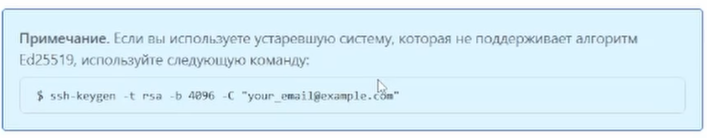
\includegraphics{./tex2pdf.-cbf55669a78d292a/image/7.PNG}
\caption{(рис. 7. Запрос ключа)}
\end{figure}

\textbf{8.} Получим SSH-ключ:

\begin{figure}
\centering
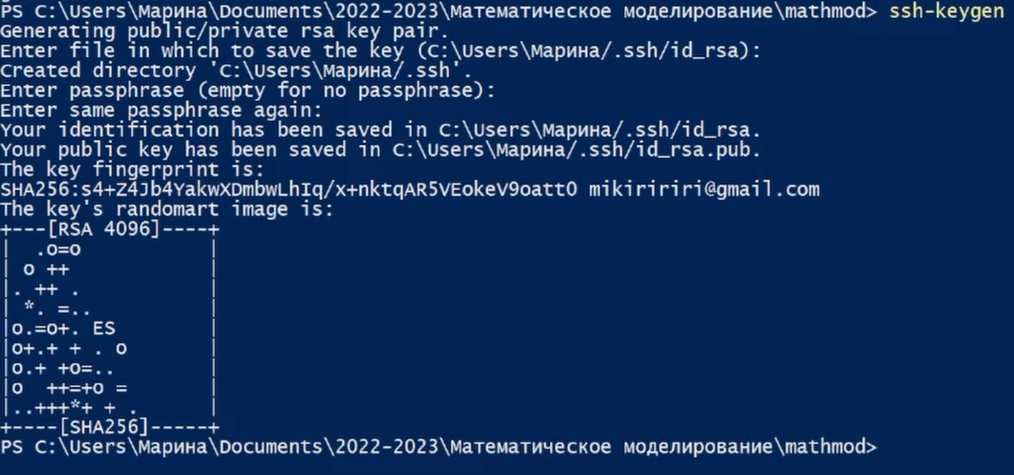
\includegraphics{./tex2pdf.-cbf55669a78d292a/image/8.PNG}
\caption{(рис. 8. Получение ключа)}
\end{figure}

\textbf{9.} Получим id SSH-ключа:

\begin{figure}
\centering
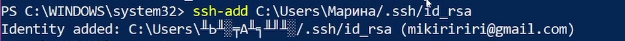
\includegraphics{./tex2pdf.-cbf55669a78d292a/image/9.PNG}
\caption{(рис. 9. Получение id ключа)}
\end{figure}

\textbf{10.} Добавим связку по SSH-ключу на сайт:

\begin{figure}
\centering
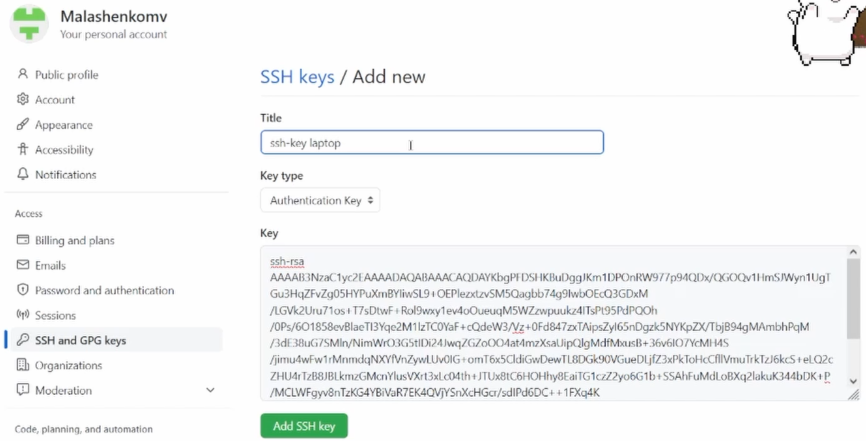
\includegraphics{./tex2pdf.-cbf55669a78d292a/image/10.PNG}
\caption{(рис. 10. Добавление ключа)}
\end{figure}

\textbf{11.} Клонируем репозиторий:

\texttt{git\ clone\ -\/-recursive\ git@github.com:malashenkomv/mathmod}

\begin{figure}
\centering
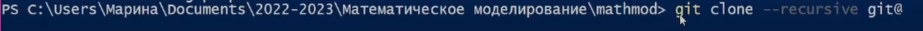
\includegraphics{./tex2pdf.-cbf55669a78d292a/image/11.PNG}
\caption{(рис. 11. Клонирование)}
\end{figure}

\textbf{12.} Репозиторий склонирован:

\begin{figure}
\centering
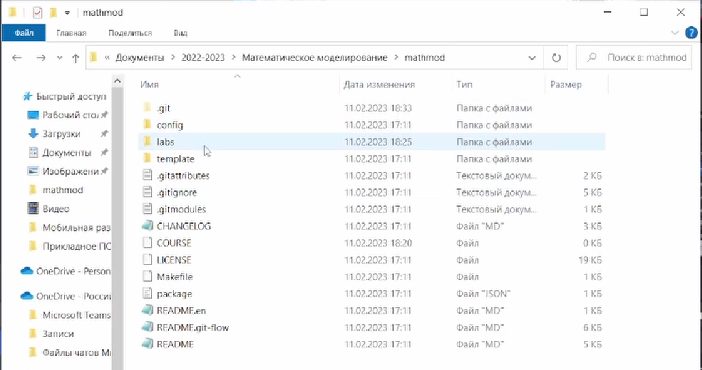
\includegraphics{./tex2pdf.-cbf55669a78d292a/image/12.PNG}
\caption{(рис. 12. Репозиторий в директории)}
\end{figure}

Создадим папку Labs с внутренней папкой Lab01. Внутри папки Lab01 папки
report и presentation.

\textbf{13.} Вид папки Lab01/report:

\begin{figure}
\centering
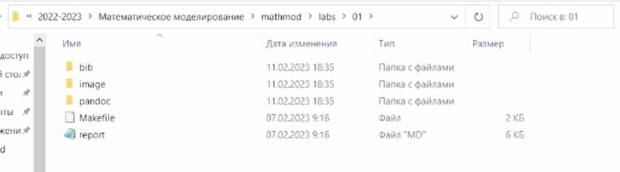
\includegraphics{./tex2pdf.-cbf55669a78d292a/image/13.PNG}
\caption{(рис. 13. Папка лабораторной работы)}
\end{figure}

\textbf{14.} Конвертируем .md файл в docx командой make:

\begin{figure}
\centering
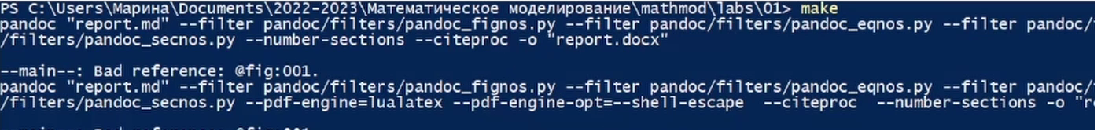
\includegraphics{./tex2pdf.-cbf55669a78d292a/image/14.PNG}
\caption{(рис. 14. Конвертация в docx)}
\end{figure}

\textbf{15.} Получили docx файл:

\begin{figure}
\centering
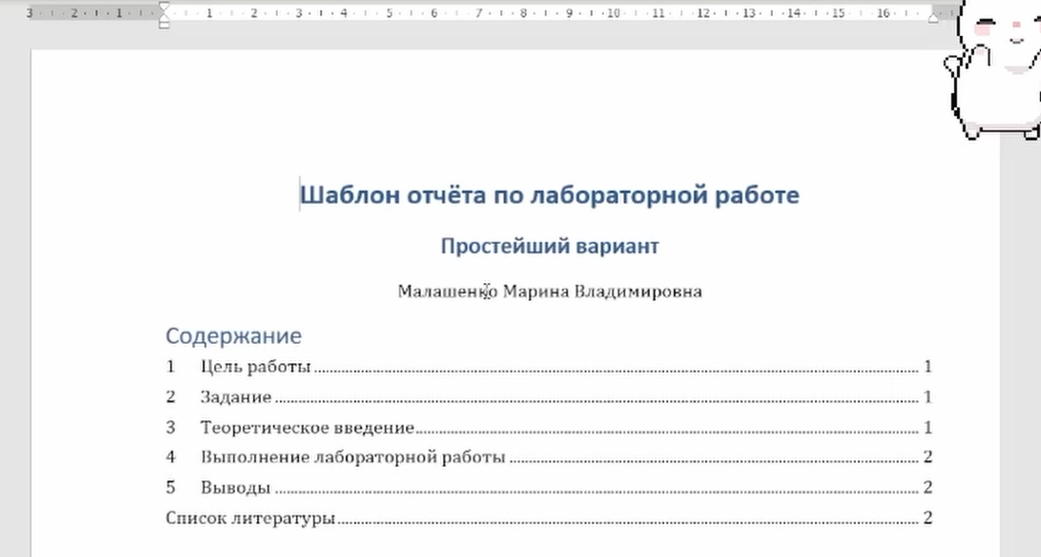
\includegraphics{./tex2pdf.-cbf55669a78d292a/image/15.PNG}
\caption{(рис. 15. Полученный docx)}
\end{figure}

\textbf{16.} Для конвертации .md файла в pdf потребуется установка TeX
Live.Установим MiKTeX как альтернативу TeX Live для LaTeX:

\begin{figure}
\centering
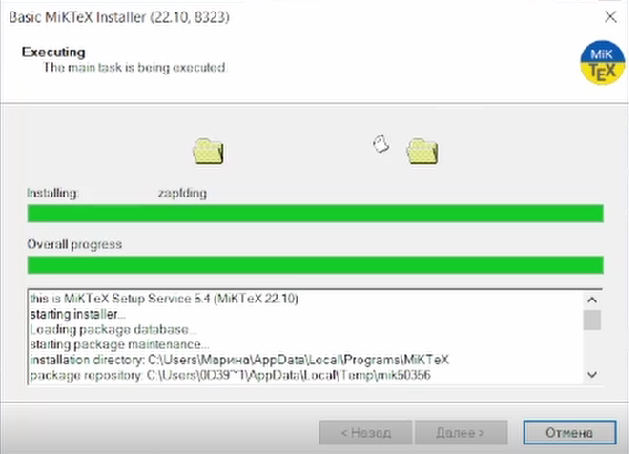
\includegraphics{./tex2pdf.-cbf55669a78d292a/image/16.PNG}
\caption{(рис. 16. MiKTeX)}
\end{figure}

\textbf{17.} Конвертируем .md файл в pdf командой:

\texttt{pandoc\ report.md\ -o\ report.pdf\ -\/-pdf-engine=lualatex\ -V\ mainfont="Times\ New\ Roman"\ -V\ sansfont="DejaVu\ Sans"\ -V\ monofont="DejaVu\ Sans\ Mono"}

\begin{figure}
\centering
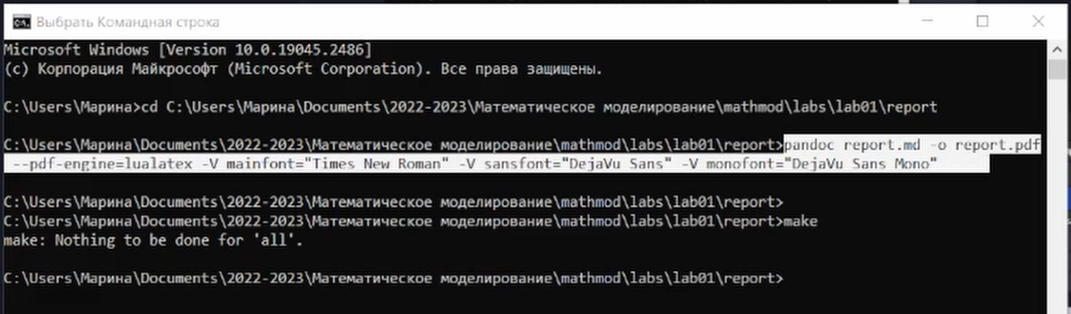
\includegraphics{./tex2pdf.-cbf55669a78d292a/image/17.PNG}
\caption{(рис. 17. Конвертация в pdf)}
\end{figure}

\textbf{18.} Получили pdf файл:

\begin{figure}
\centering

\includegraphics{./tex2pdf.-cbf55669a78d292a/image/18.PNG}
\caption{(рис. 18. Полученный pdf)}
\end{figure}

\textbf{19.} Итоговый вид папки отчета лабораторной работы:

\begin{figure}
\centering
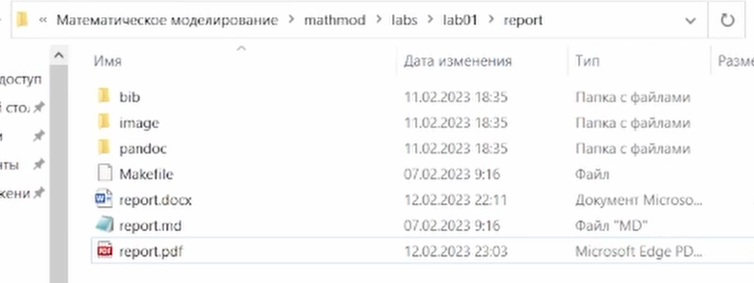
\includegraphics{./tex2pdf.-cbf55669a78d292a/image/19.PNG}
\caption{(рис. 19. Папка отчета лабораторной работы)}
\end{figure}

\textbf{20.} Конвертируем .md файл презентации в pdf презентации
командой:

\texttt{pandoc\ presentation.md\ -o\ presentation.pdf\ —-pdf-engine=lualatex\ -V\ mainfont="Times\ New\ Roman"\ -V\ sansfont="DejaVu\ Sans"\ -V\ monofont="DejaVu\ Sans\ Mono"\ -t\ beamer\ —-slide-level=2}

\begin{figure}
\centering
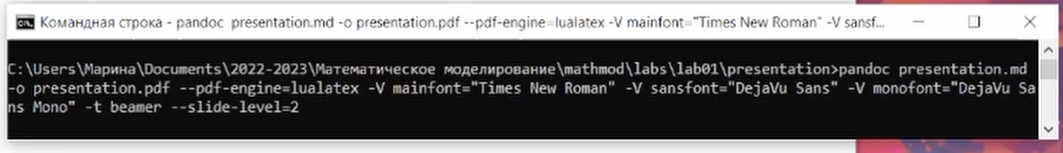
\includegraphics{./tex2pdf.-cbf55669a78d292a/image/20.PNG}
\caption{(рис. 20. Конвертация презентации)}
\end{figure}

\textbf{21.} Получили pdf файл презентации:

\begin{figure}
\centering
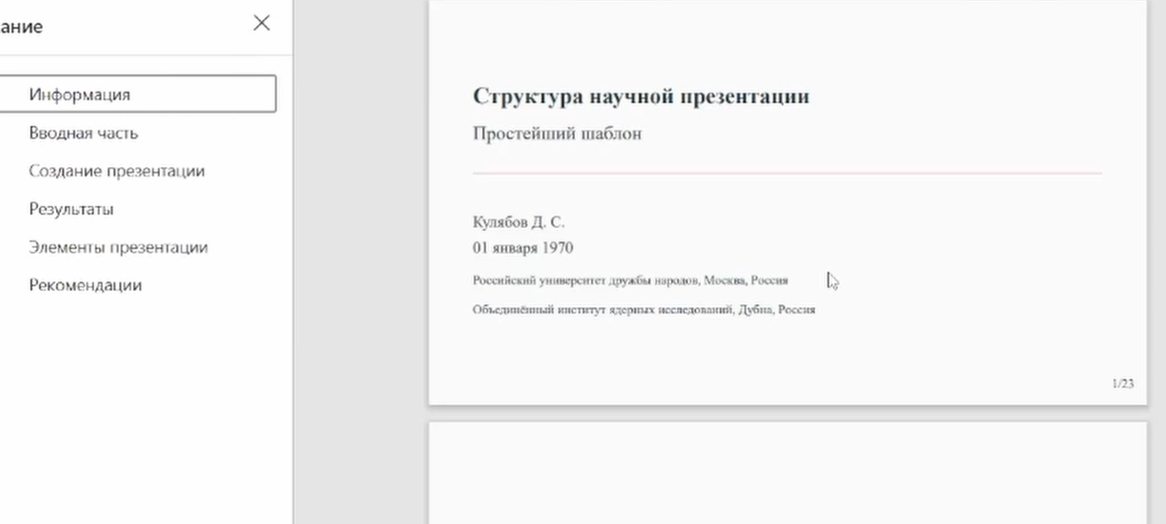
\includegraphics{./tex2pdf.-cbf55669a78d292a/image/21.PNG}
\caption{(рис. 21. Полученный pdf презентации)}
\end{figure}

\textbf{22.} Отправим все изменения на GitHub командами:

{} {} {(рис. 22. Отправка изменений)}

\textbf{23.} Изменения успешно отправлены в репозиторий с указанным
коммитом.

\begin{figure}
\centering
{(рис. 23. Репозиторий)}
\caption{(рис. 23. Репозиторий)}
\end{figure}

\hypertarget{ux432ux44bux432ux43eux434}{%
\chapter{Вывод}\label{ux432ux44bux432ux43eux434}}

Мы настроили рабочее пространство для лабораторной работы. Изучили
систему контроля версий Git и язык разметки Markdown.

\hypertarget{ux441ux43fux438ux441ux43eux43a-ux43bux438ux442ux435ux440ux430ux442ux443ux440ux44b.-ux431ux438ux431ux43bux438ux43eux433ux440ux430ux444ux438ux44f}{%
\chapter{Список литературы.
Библиография}\label{ux441ux43fux438ux441ux43eux43a-ux43bux438ux442ux435ux440ux430ux442ux443ux440ux44b.-ux431ux438ux431ux43bux438ux43eux433ux440ux430ux444ux438ux44f}}

\begin{itemize}
\item
  Документация по Git: https://git-scm.com/book/ru/v2
\item
  Документация по Markdown:
  https://learn.microsoft.com/ru-ru/contribute/markdown-reference
\item
  Документация по MiKTeX:
  https://kpfu.ru/staff\_files/F2077692752/Inst\_MiKTeX.pdf
\end{itemize}

\printbibliography

\end{document}
